\section{Current Drive}
\begin{frame} {Plasma Rotation}
    \begin{itemize}
        \item Neutral beams are injected into the plasma with toroidal velocity causes plasma to spin.
        \item The spin of plasma introduces a centrifugal force, hence breaking the Grad-Shafranov equation.
    \end{itemize}
    \begin{figure}
        \centering
        \begin{subfigure}{0.45\textwidth}
            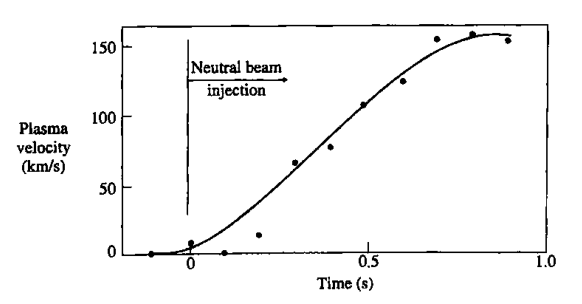
\includegraphics[width=\textwidth]{figures/plasma-velocity.png}
            \caption{Plasma velocity during neutral beam injection as measured by the Doppler shift of the impurity spectral lines (JET).}
        \end{subfigure}%
        \begin{subfigure}{0.45\textwidth}
            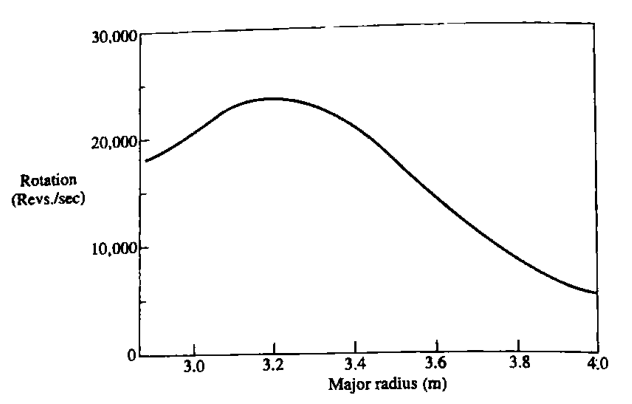
\includegraphics[width=\textwidth]{figures/rotation-velocity.png}
            \caption{Typical radial profile of toroidal rotation of a plasma spun by neotral beam injection (JET).}
        \end{subfigure}
        \label{fig:centrifugal-effect}
    \end{figure}
\end{frame}

\begin{frame} {Current Drive}
    \begin{itemize}
        \item \textbf{Neutral beam injection}: ions in the plasma center will be accelerated, hence creating a toroidal current.
        \item \textbf{Lower hybrid current drive}: the energy of low waves with high $v_\parallel$ is deposited into the plasma by Landau damping. Creating a toroidal current. High efficiency in the outer half of the plasma.
        \item \textbf{Fast wave electron current drive}: uses fast magnetosonic waves in the ion cyclotron frequency range. Similar to lower hybrid waves, the energy is deposited into plasma by Landau damping. The force on the electrons is due to the $E_\parallel$, $\grad_\parallel B$ of the waves and the magnetic moment of the electrons. Transit time magnetic pumping (TTMP).
        \item \textbf{Electron cyclotron current drive}: heating only those electrons circulating in a particular toroidal direction. It is to accelerate electrons primarily in the perpendicular direction. Good for control of mhd instabilities.
        \item \textbf{Fast wave minority ion current drive}: Similar to electron cyclotron current drive, but this time we heat up ion.
    \end{itemize}
\end{frame}

\begin{frame}{Current Drive - Figure}
    \begin{figure}
        \centering
        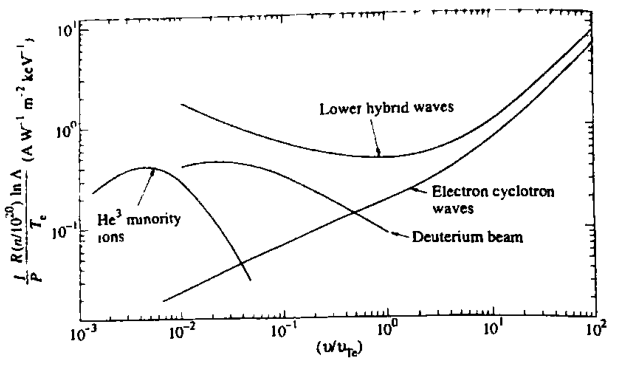
\includegraphics[width=0.65\textwidth]{figures/current-drive.png}
        \caption{Comparison of theoretical current drive effecicieny for (i) deuterium beams injected into a D-T plasma; (ii) Landau damping of lower hybrid waves. (iii) electron cyclotron waves, and (iv) He$^3$ minority ions in a deuterium plasma. The scale gives the ratio of the total current $I$(\unit{\A}) to the otal power injected, $P$(\unit{\W}), into a tokamak plasma of major radius $R$(\unit{\m}), density $n(10^{20})$\unit{\m\tothe{-3}}, and temperature $T_e$(\unit{\kilo\eV}). $v$ is the wave phase velocity, or beam ion velocity, and $v_{T_e}$ is the electron thermal velocity.}
        \label{fig:}
    \end{figure}
\end{frame}